\documentclass[10pt,a4paper]{article}\usepackage[]{graphicx}\usepackage[]{color}
%% maxwidth is the original width if it is less than linewidth
%% otherwise use linewidth (to make sure the graphics do not exceed the margin)
\makeatletter
\def\maxwidth{ %
  \ifdim\Gin@nat@width>\linewidth
    \linewidth
  \else
    \Gin@nat@width
  \fi
}
\makeatother

\definecolor{fgcolor}{rgb}{0.345, 0.345, 0.345}
\newcommand{\hlnum}[1]{\textcolor[rgb]{0.686,0.059,0.569}{#1}}%
\newcommand{\hlstr}[1]{\textcolor[rgb]{0.192,0.494,0.8}{#1}}%
\newcommand{\hlcom}[1]{\textcolor[rgb]{0.678,0.584,0.686}{\textit{#1}}}%
\newcommand{\hlopt}[1]{\textcolor[rgb]{0,0,0}{#1}}%
\newcommand{\hlstd}[1]{\textcolor[rgb]{0.345,0.345,0.345}{#1}}%
\newcommand{\hlkwa}[1]{\textcolor[rgb]{0.161,0.373,0.58}{\textbf{#1}}}%
\newcommand{\hlkwb}[1]{\textcolor[rgb]{0.69,0.353,0.396}{#1}}%
\newcommand{\hlkwc}[1]{\textcolor[rgb]{0.333,0.667,0.333}{#1}}%
\newcommand{\hlkwd}[1]{\textcolor[rgb]{0.737,0.353,0.396}{\textbf{#1}}}%

\usepackage{framed}
\makeatletter
\newenvironment{kframe}{%
 \def\at@end@of@kframe{}%
 \ifinner\ifhmode%
  \def\at@end@of@kframe{\end{minipage}}%
  \begin{minipage}{\columnwidth}%
 \fi\fi%
 \def\FrameCommand##1{\hskip\@totalleftmargin \hskip-\fboxsep
 \colorbox{shadecolor}{##1}\hskip-\fboxsep
     % There is no \\@totalrightmargin, so:
     \hskip-\linewidth \hskip-\@totalleftmargin \hskip\columnwidth}%
 \MakeFramed {\advance\hsize-\width
   \@totalleftmargin\z@ \linewidth\hsize
   \@setminipage}}%
 {\par\unskip\endMakeFramed%
 \at@end@of@kframe}
\makeatother

\definecolor{shadecolor}{rgb}{.97, .97, .97}
\definecolor{messagecolor}{rgb}{0, 0, 0}
\definecolor{warningcolor}{rgb}{1, 0, 1}
\definecolor{errorcolor}{rgb}{1, 0, 0}
\newenvironment{knitrout}{}{} % an empty environment to be redefined in TeX

\usepackage{alltt}

\usepackage[T1]{fontenc}
\usepackage[polish]{babel}
\usepackage[cp1250]{inputenc}
\usepackage{amsmath}
\usepackage{amsfonts}
\usepackage{graphicx}
\usepackage{setspace}
\usepackage{savesym}
\savesymbol{arc}
\usepackage{color}
\usepackage{xcolor}
\usepackage{pict2e}
\usepackage{epstopdf}
\usepackage{geometry}

\newgeometry{tmargin=1.5cm, bmargin=1.5cm, lmargin=1.5cm, rmargin=1.5cm}
\pagestyle{empty}
\linespread{1.2}
\IfFileExists{upquote.sty}{\usepackage{upquote}}{}

\begin{document}

\section*{\centering PRACA DOMOWA 1\\ ASC - 04 maja 2014r.\\ \textbf{MARTA SOMMER} -- BSMAD -- 237503}

\subsection*{\underline{\textbf{Zadanie 4.}}}

\subsubsection*{\textbf{a)}}

Generuj� $500$ liczb z modelu $MA(1)$:

$$
X_t=Z_t-0,8\cdot Z_{t-1},
$$
gdzie $Z_t$ - bia�y szum o rozk�adzie $\mathcal{N}(0,1)$.

\begin{knitrout}
\definecolor{shadecolor}{rgb}{0.969, 0.969, 0.969}\color{fgcolor}\begin{kframe}
\begin{alltt}
\hlkwd{set.seed}\hlstd{(}\hlnum{400}\hlstd{)}
\hlstd{zt} \hlkwb{<-} \hlkwd{rnorm}\hlstd{(}\hlnum{501}\hlstd{)}
\hlstd{xt} \hlkwb{<-} \hlkwd{numeric}\hlstd{(}\hlnum{500}\hlstd{)}

\hlkwa{for} \hlstd{(i} \hlkwa{in} \hlnum{1}\hlopt{:}\hlnum{500}\hlstd{) \{}
    \hlstd{xt[i]} \hlkwb{<-} \hlstd{zt[i} \hlopt{+} \hlnum{1}\hlstd{]} \hlopt{-} \hlnum{0.8} \hlopt{*} \hlstd{zt[i]}
\hlstd{\}}

\hlstd{t} \hlkwb{<-} \hlkwd{ts}\hlstd{(xt)}
\hlkwd{plot}\hlstd{(t)}
\end{alltt}
\end{kframe}

{\centering 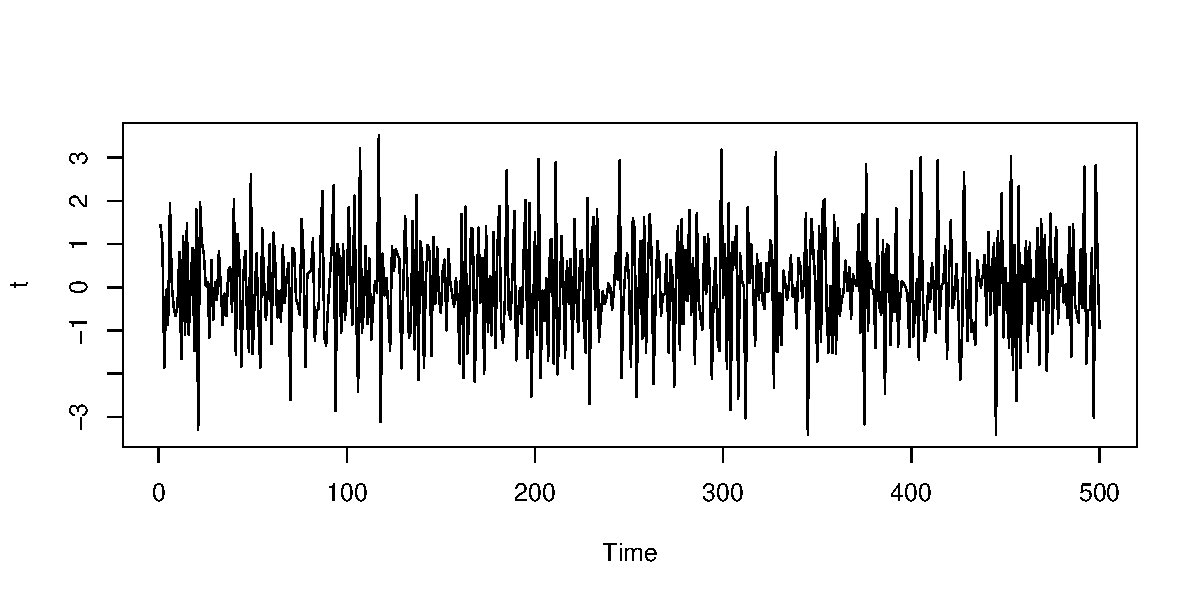
\includegraphics[width=\maxwidth]{figure/unnamed-chunk-1} 

}



\end{knitrout}


\subsubsection*{\textbf{b)}}

Wyznaczam funkcj� autokorelacji:

\begin{knitrout}
\definecolor{shadecolor}{rgb}{0.969, 0.969, 0.969}\color{fgcolor}\begin{kframe}
\begin{alltt}
\hlkwd{acf}\hlstd{(t)}
\end{alltt}
\end{kframe}

{\centering 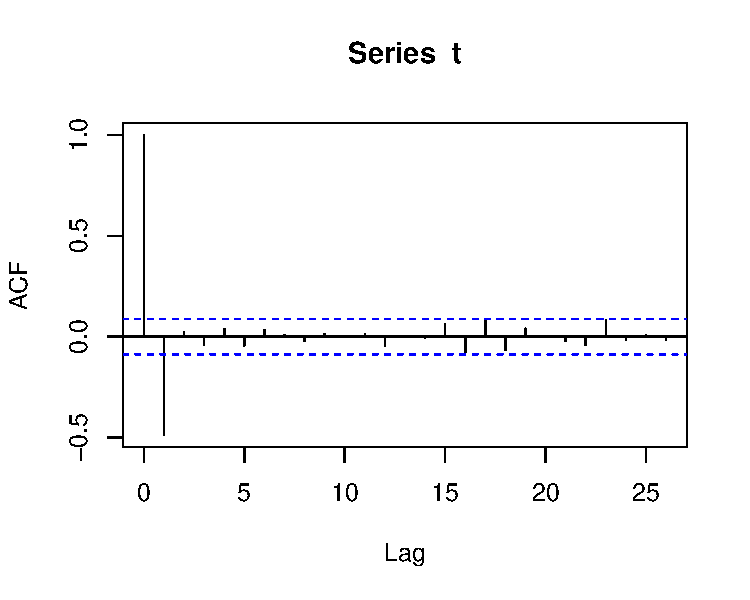
\includegraphics[width=\maxwidth]{figure/unnamed-chunk-2} 

}



\end{knitrout}


Z wykresu wyra�nie wida�, �e jest to proces MA(1).

\subsubsection*{\textbf{c)}}

Wyznaczam zale�no�� $x\sim lag1+lag2$:

\begin{knitrout}
\definecolor{shadecolor}{rgb}{0.969, 0.969, 0.969}\color{fgcolor}\begin{kframe}
\begin{alltt}
\hlkwd{library}\hlstd{(}\hlstr{"quantmod"}\hlstd{)}

\hlstd{lag1} \hlkwb{<-} \hlkwd{Lag}\hlstd{(xt)}
\hlstd{lag2} \hlkwb{<-} \hlkwd{Lag}\hlstd{(xt,} \hlkwc{k} \hlstd{=} \hlnum{2}\hlstd{)}

\hlstd{l2} \hlkwb{<-} \hlkwd{lm}\hlstd{(xt} \hlopt{~} \hlstd{lag1} \hlopt{+} \hlstd{lag2)}

\hlkwd{summary}\hlstd{(l2)}
\end{alltt}
\begin{verbatim}
## 
## Call:
## lm(formula = xt ~ lag1 + lag2)
## 
## Residuals:
##    Min     1Q Median     3Q    Max 
## -2.976 -0.704 -0.049  0.665  3.494 
## 
## Coefficients:
##             Estimate Std. Error t value Pr(>|t|)    
## (Intercept) -0.00535    0.04835   -0.11     0.91    
## lag1        -0.62963    0.04300  -14.64  < 2e-16 ***
## lag2        -0.28424    0.04295   -6.62  9.5e-11 ***
## ---
## Signif. codes:  0 '***' 0.001 '**' 0.01 '*' 0.05 '.' 0.1 ' ' 1
## 
## Residual standard error: 1.08 on 495 degrees of freedom
##   (2 observations deleted due to missingness)
## Multiple R-squared:  0.303,	Adjusted R-squared:   0.3 
## F-statistic:  107 on 2 and 495 DF,  p-value: <2e-16
\end{verbatim}
\end{kframe}
\end{knitrout}


Z $summary()$ mo�emy odczyta�, �e warto�� wsp�czynnika kierunkowego przy $lag1$ to $-0,62963$, a przy $lag2$ to $-0,28424$, a odpowiadaj�ce im $p-value$ to $< 2e-16$ oraz $9,5e-11$.

\subsubsection*{\textbf{d)}}

Buduj� model $x\sim lag1$:

\begin{knitrout}
\definecolor{shadecolor}{rgb}{0.969, 0.969, 0.969}\color{fgcolor}\begin{kframe}
\begin{alltt}
\hlstd{l1} \hlkwb{<-} \hlkwd{lm}\hlstd{(xt} \hlopt{~} \hlstd{lag1)}
\hlkwd{summary}\hlstd{(l1)}
\end{alltt}
\begin{verbatim}
## 
## Call:
## lm(formula = xt ~ lag1)
## 
## Residuals:
##    Min     1Q Median     3Q    Max 
## -3.022 -0.757 -0.006  0.758  3.469 
## 
## Coefficients:
##             Estimate Std. Error t value Pr(>|t|)    
## (Intercept)  -0.0020     0.0504   -0.04     0.97    
## lag1         -0.4879     0.0391  -12.47   <2e-16 ***
## ---
## Signif. codes:  0 '***' 0.001 '**' 0.01 '*' 0.05 '.' 0.1 ' ' 1
## 
## Residual standard error: 1.13 on 497 degrees of freedom
##   (1 observation deleted due to missingness)
## Multiple R-squared:  0.238,	Adjusted R-squared:  0.237 
## F-statistic:  156 on 1 and 497 DF,  p-value: <2e-16
\end{verbatim}
\end{kframe}
\end{knitrout}


Wsp�czynnik kierunkowy przy $lag1$ (-0.4879) jest to teoretyczny wsp�czynnik $pacf(1)=\alpha(1)=\dfrac{\gamma(1)}{\gamma(0)}$. Policzmy~to:

\begin{eqnarray*}
\gamma(0)&=&<X_t,X_t>=<Z_t-0,8\cdot Z_{t-1},Z_t-0,8\cdot Z_{t-1}>=1+(0,8)^2=1,64 \\
\gamma(1)&=&<X_t,X_{t-1}>=<Z_t-0,8\cdot Z_{t-1},Z_{t-1}-0,8\cdot Z_{t-2}>=-0,8\\
\dfrac{\gamma(1)}{\gamma(0)}&=&\dfrac{-0,8}{1,64}\approx -0,49
\end{eqnarray*}

Nasza warto�� teoretyczna mie�ci si� w granicach b��du empirycznej, wi�c wynik wyszed� nam sensowny.

\subsection*{\underline{\textbf{Zadanie 5.}}}

\subsubsection*{\textbf{a)}}

Generuj� $500$ liczb z modelu $AR(1)$:

$$
X_t=0,8\cdot X_{t-1}+\varepsilon_{t},
$$
gdzie $X_0=1$, $\varepsilon_t \sim \mathcal{N}(0,0.1)$.

\begin{knitrout}
\definecolor{shadecolor}{rgb}{0.969, 0.969, 0.969}\color{fgcolor}\begin{kframe}
\begin{alltt}
\hlkwd{set.seed}\hlstd{(}\hlnum{500}\hlstd{)}
\hlstd{x0} \hlkwb{<-} \hlnum{1}
\hlstd{eps} \hlkwb{<-} \hlkwd{rnorm}\hlstd{(}\hlnum{500}\hlstd{,} \hlnum{0}\hlstd{,} \hlnum{0.1}\hlstd{)}
\hlstd{xt} \hlkwb{<-} \hlkwd{numeric}\hlstd{(}\hlnum{500}\hlstd{)}
\hlstd{xt[}\hlnum{1}\hlstd{]} \hlkwb{<-} \hlstd{x0}
\hlkwa{for} \hlstd{(i} \hlkwa{in} \hlnum{2}\hlopt{:}\hlnum{500}\hlstd{) \{}
    \hlstd{xt[i]} \hlkwb{<-} \hlstd{xt[i} \hlopt{-} \hlnum{1}\hlstd{]} \hlopt{*} \hlnum{0.8} \hlopt{+} \hlstd{eps[i]}
\hlstd{\}}
\end{alltt}
\end{kframe}
\end{knitrout}


\subsubsection*{\textbf{b)}}

\begin{knitrout}
\definecolor{shadecolor}{rgb}{0.969, 0.969, 0.969}\color{fgcolor}\begin{kframe}
\begin{alltt}
\hlkwd{plot}\hlstd{(xt,} \hlkwc{type} \hlstd{=} \hlstr{"l"}\hlstd{)}
\end{alltt}
\end{kframe}

{\centering 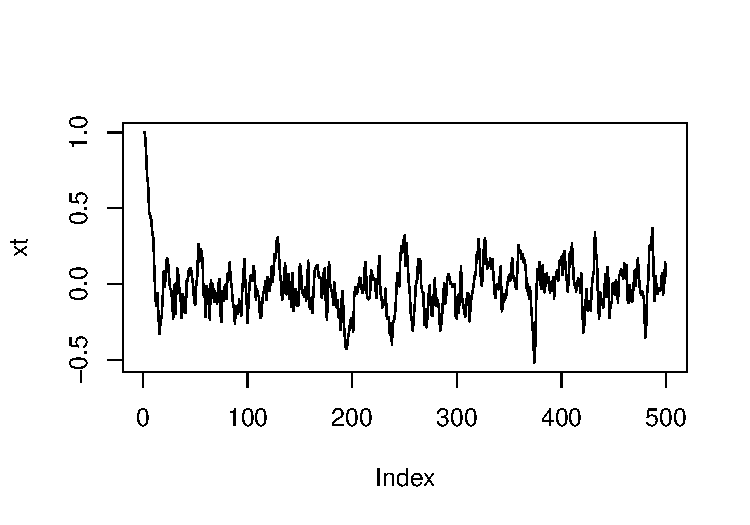
\includegraphics[width=\maxwidth]{figure/unnamed-chunk-61} 

}


\begin{kframe}\begin{alltt}
\hlkwd{pacf}\hlstd{(xt)}
\end{alltt}
\end{kframe}

{\centering 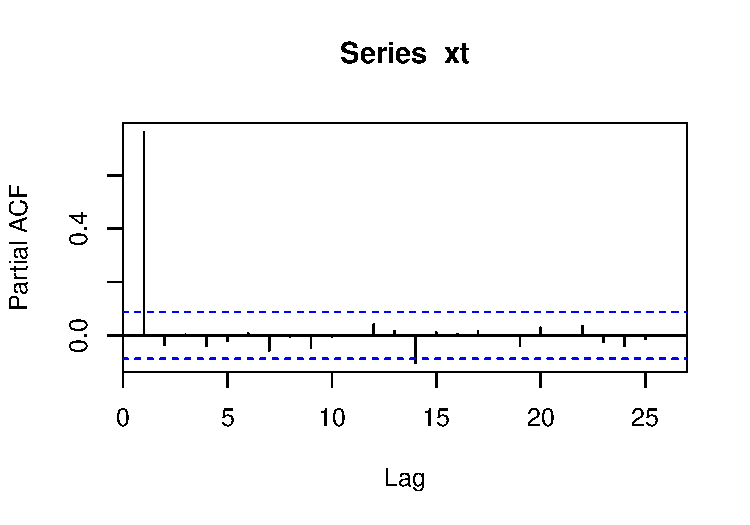
\includegraphics[width=\maxwidth]{figure/unnamed-chunk-62} 

}


\begin{kframe}\begin{alltt}
\hlkwd{acf}\hlstd{(xt)}
\end{alltt}
\end{kframe}

{\centering 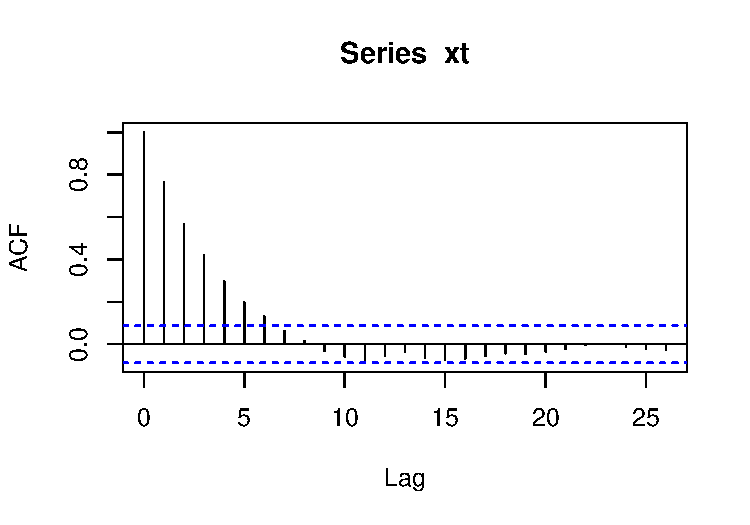
\includegraphics[width=\maxwidth]{figure/unnamed-chunk-63} 

}



\end{knitrout}


Z wykresu PACF wida� wyra�nie, �e jest to proces $AR(1)$.

\subsubsection*{\textbf{c)}}

\begin{knitrout}
\definecolor{shadecolor}{rgb}{0.969, 0.969, 0.969}\color{fgcolor}\begin{kframe}
\begin{alltt}
\hlstd{sr} \hlkwb{<-} \hlkwd{mean}\hlstd{(xt)}
\hlstd{gamma0} \hlkwb{<-} \hlstd{(}\hlkwd{sum}\hlstd{((xt} \hlopt{-} \hlstd{sr)}\hlopt{^}\hlnum{2}\hlstd{))}\hlopt{/}\hlnum{500}
\hlstd{gamma1} \hlkwb{<-} \hlstd{(}\hlkwd{sum}\hlstd{((xt[}\hlnum{1}\hlopt{:}\hlnum{499}\hlstd{]} \hlopt{-} \hlstd{sr)} \hlopt{*} \hlstd{(xt[}\hlnum{2}\hlopt{:}\hlnum{500}\hlstd{]} \hlopt{-} \hlstd{sr)))}\hlopt{/}\hlnum{500}
\hlstd{gamma2} \hlkwb{<-} \hlstd{(}\hlkwd{sum}\hlstd{((xt[}\hlnum{1}\hlopt{:}\hlnum{498}\hlstd{]} \hlopt{-} \hlstd{sr)} \hlopt{*} \hlstd{(xt[}\hlnum{3}\hlopt{:}\hlnum{500}\hlstd{]} \hlopt{-} \hlstd{sr)))}\hlopt{/}\hlnum{500}
\hlstd{gamma3} \hlkwb{<-} \hlstd{(}\hlkwd{sum}\hlstd{((xt[}\hlnum{1}\hlopt{:}\hlnum{497}\hlstd{]} \hlopt{-} \hlstd{sr)} \hlopt{*} \hlstd{(xt[}\hlnum{4}\hlopt{:}\hlnum{500}\hlstd{]} \hlopt{-} \hlstd{sr)))}\hlopt{/}\hlnum{500}

\hlstd{ro0} \hlkwb{<-} \hlnum{1}
\hlstd{ro1} \hlkwb{<-} \hlstd{gamma1}\hlopt{/}\hlstd{gamma0}
\hlstd{ro2} \hlkwb{<-} \hlstd{gamma2}\hlopt{/}\hlstd{gamma0}
\hlstd{ro3} \hlkwb{<-} \hlstd{gamma3}\hlopt{/}\hlstd{gamma0}

\hlstd{ro1}\hlopt{/}\hlstd{ro0}
\end{alltt}
\begin{verbatim}
## [1] 0.7618
\end{verbatim}
\begin{alltt}
\hlstd{ro2}\hlopt{/}\hlstd{ro1}
\end{alltt}
\begin{verbatim}
## [1] 0.7422
\end{verbatim}
\begin{alltt}
\hlstd{ro3}\hlopt{/}\hlstd{ro2}
\end{alltt}
\begin{verbatim}
## [1] 0.7427
\end{verbatim}
\end{kframe}
\end{knitrout}


Stosunek kolejnych wsp�czynnik�w korelacji jest praktycznie identyczny. Wskazuje na to, �e funkcja autokorelacji w ka�dym kroku maleje tyle samo razy.

\subsubsection*{\textbf{d)}}

\begin{knitrout}
\definecolor{shadecolor}{rgb}{0.969, 0.969, 0.969}\color{fgcolor}\begin{kframe}
\begin{alltt}
\hlstd{lag1} \hlkwb{<-} \hlkwd{Lag}\hlstd{(xt)}
\hlstd{l} \hlkwb{<-} \hlkwd{lm}\hlstd{(xt} \hlopt{~} \hlstd{lag1)}
\hlkwd{summary}\hlstd{(l)}
\end{alltt}
\begin{verbatim}
## 
## Call:
## lm(formula = xt ~ lag1)
## 
## Residuals:
##      Min       1Q   Median       3Q      Max 
## -0.26354 -0.06522 -0.00031  0.07164  0.28113 
## 
## Coefficients:
##             Estimate Std. Error t value Pr(>|t|)    
## (Intercept) -0.00530    0.00456   -1.16     0.25    
## lag1         0.76206    0.02651   28.74   <2e-16 ***
## ---
## Signif. codes:  0 '***' 0.001 '**' 0.01 '*' 0.05 '.' 0.1 ' ' 1
## 
## Residual standard error: 0.102 on 497 degrees of freedom
##   (1 observation deleted due to missingness)
## Multiple R-squared:  0.624,	Adjusted R-squared:  0.624 
## F-statistic:  826 on 1 and 497 DF,  p-value: <2e-16
\end{verbatim}
\end{kframe}
\end{knitrout}


Wsp�czynnik kierunkowy prostej wynosi $0,76206$. Teoretycznie powinni�my otrzyma�: $pacf(1)=\alpha(1)=\dfrac{\gamma(1)}{\gamma(0)}$. Policzmy~to:

\begin{eqnarray*}
\gamma(0)&=&<X_t,X_t>=<0.8\cdot X_{t-1}+\varepsilon_{t},X_t>=0.8\cdot\gamma(1)+<\varepsilon_t,0.8\cdot X_{t-1}+\varepsilon_{t}>= 0.8\cdot\gamma(1)+\sigma^2\\
\gamma(1)&=&<X_t,X_{t-1}>=<0.8\cdot X_{t-1}+\varepsilon_{t},X_{t-1}>=0.8\cdot\gamma(0)\\
\gamma(0)&=&(0.8)^2\cdot\gamma(0)+\sigma^2\\
\gamma(0)&=&\dfrac{\sigma^2}{0.36}\\
\gamma(1)&=&0.8\cdot\dfrac{\sigma^2}{0.36}\\
\dfrac{\gamma(1)}{\gamma(0)}&=&\dfrac{0.8\cdot\sigma^2}{0.36}\cdot\dfrac{0.36}{\sigma^2}=0.8\\
\end{eqnarray*}

Teoretycznie wysz�o $0,8$, a empirycznie $0,76206$. Tak wi�c podobnie, w granicy b��du.

\subsubsection*{\textbf{e)}}

Zmienimy model na: 

$$
X_t=X_{t-1}+\varepsilon_{t},
$$
gdzie $X_0=1$, $\varepsilon_t \sim \mathcal{N}(0,0.1)$.

\begin{knitrout}
\definecolor{shadecolor}{rgb}{0.969, 0.969, 0.969}\color{fgcolor}\begin{kframe}
\begin{alltt}
\hlstd{x0} \hlkwb{<-} \hlnum{1}
\hlstd{eps} \hlkwb{<-} \hlkwd{rnorm}\hlstd{(}\hlnum{500}\hlstd{,} \hlnum{0}\hlstd{,} \hlnum{0.1}\hlstd{)}
\hlstd{xt} \hlkwb{<-} \hlkwd{numeric}\hlstd{(}\hlnum{500}\hlstd{)}
\hlstd{xt[}\hlnum{1}\hlstd{]} \hlkwb{<-} \hlstd{x0}
\hlkwa{for} \hlstd{(i} \hlkwa{in} \hlnum{2}\hlopt{:}\hlnum{500}\hlstd{) \{}
    \hlstd{xt[i]} \hlkwb{<-} \hlstd{xt[i} \hlopt{-} \hlnum{1}\hlstd{]} \hlopt{+} \hlstd{eps[i]}
\hlstd{\}}

\hlkwd{plot}\hlstd{(xt,} \hlkwc{type} \hlstd{=} \hlstr{"l"}\hlstd{)}
\end{alltt}
\end{kframe}

{\centering 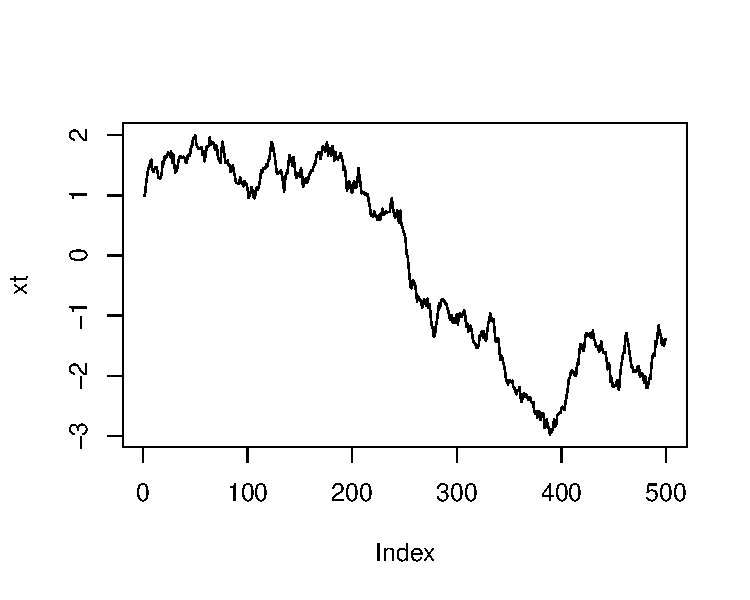
\includegraphics[width=\maxwidth]{figure/unnamed-chunk-91} 

}


\begin{kframe}\begin{alltt}
\hlkwd{pacf}\hlstd{(xt)}
\end{alltt}
\end{kframe}

{\centering 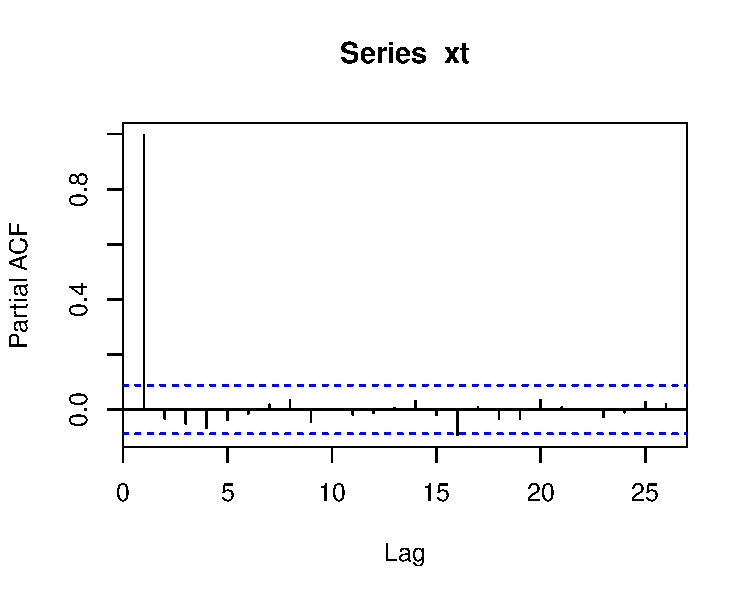
\includegraphics[width=\maxwidth]{figure/unnamed-chunk-92} 

}


\begin{kframe}\begin{alltt}
\hlkwd{acf}\hlstd{(xt)}
\end{alltt}
\end{kframe}

{\centering 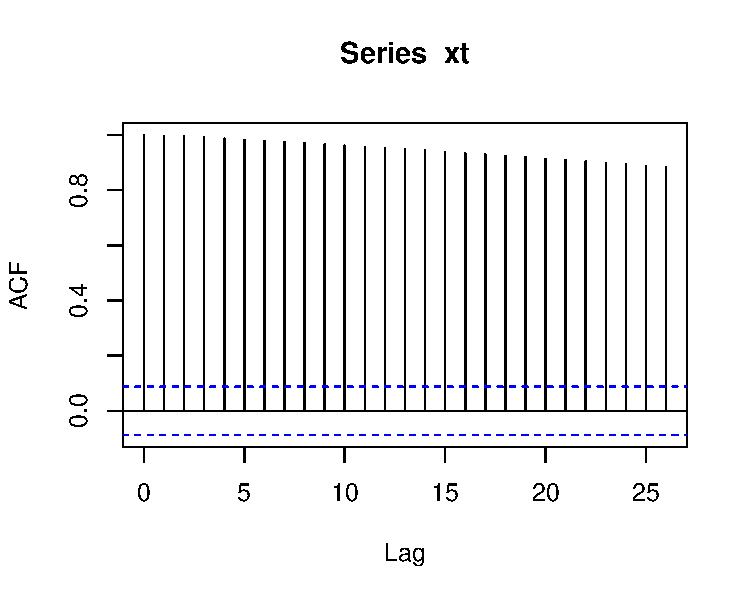
\includegraphics[width=\maxwidth]{figure/unnamed-chunk-93} 

}



\end{knitrout}


Z wykres�w wyra�nie wida�, �e jest to zwyk�e b��dzenie losowe.

\end{document}


